% SIAM Article Template
\documentclass[review,onefignum,onetabnum]{siamart190516}

% Information that is shared between the article and the supplement
% (title and author information, macros, packages, etc.) goes into
% ex_shared.tex. If there is no supplement, this file can be included
% directly.

% SIAM Shared Information Template
% This is information that is shared between the main document and any
% supplement. If no supplement is required, then this information can
% be included directly in the main document.


% Packages and macros go here
\usepackage{lipsum}
\usepackage{amsfonts}
\usepackage{graphicx}
\usepackage{epstopdf}
\usepackage{algorithmic}
\usepackage{bookmark}
\ifpdf
  \DeclareGraphicsExtensions{.eps,.pdf,.png,.jpg}
\else
  \DeclareGraphicsExtensions{.eps}
\fi

% Add a serial/Oxford comma by default.
\newcommand{\creflastconjunction}{, and~}

% Used for creating new theorem and remark environments
\newsiamremark{remark}{Remark}
\newsiamremark{hypothesis}{Hypothesis}
\crefname{hypothesis}{Hypothesis}{Hypotheses}
\newsiamthm{claim}{Claim}


% Title. If the supplement option is on, then "Supplementary Material"
% is automatically inserted before the title.
\title{18.335 Final Project Report}
\author{Juan M Ortiz}


\usepackage{amsopn}
\DeclareMathOperator{\diag}{diag}

% Packages
\usepackage{enumitem}
\usepackage{float}

% Optional PDF information
\ifpdf
\hypersetup{
  pdftitle={18.335 Final Project Report},
  pdfauthor={Juan M Ortiz}
}
\fi

\begin{document}
\maketitle

\section{Introduction}
Along with the numerous benefits that we have come to enjoy in our transition to the Digital Age
have come a plethora of technical challenges. In particular, the rise in the prominence
of the role that data plays in our services has forced us to invent efficient solutions 
to challenges related to storing, retrieving, processing, and transmitting various types of 
data. One of the most common types of data that we utilize in both computer and mobile environments
is that of images. As such, there has been a lot of research in the field of image compression.
Although the problem of compressing images falls within the general problem of compressing arbitrary
raw binary data, we can greatly improve our performance by designing encoders that take 
advantage of the statistical properties that images posses. Through the use of our domain-specific
knowledge about how images are composed as well as how we perceive images, 
modern compression algorithms are able to remove a great deal of redundancies
so as to create much smaller representations that are able to be decoded into 
good reconstructions of the originals in accordance to human visual perception.

\subsection{Compression Principles}

Today, the majority of methods utilized in image compression are based on the
principles of \textbf{entropy coding} and \textbf{transform coding}. 

The first, entropy coding, refers to a type of lossless compression scheme which is not
dependent on the medium to which it is applied. Entropy coding aims to reduce
the size of data processed by defining a mapping between the original symbols/patterns of 
the data to one in which frequently occurring symbols/patterns are represented 
using few bits and those that occur rarely are represented with more bits.
The two most common algorithms used for entropy coding are Huffman coding and
Arithmetic coding. A more detail overview of Huffman coding will be given in \textbf{Section 2}. On the other hand, transform coding refers to a technique utilized when dealing
with natural data sources such as images and audio. The main idea behind transform
coding is to utilize a linear process to convert the original representation of
the data to one in which the most relevant information is contained within
a few coefficients. On its own, a naive transform coding approach is lossless and 
does not significantly reduce the information needed to encode the original data. However,
the new representation along with domain knowledge about the data being encoded 
enables us to keep only the most relevant information to recreate something that is mostly
faithful with the original but is much smaller. The most widely used transform coding algorithm when
dealing with image compression is that of the discrete cosine transform (DCT) which
will be further described in \textbf{Section 2}. Additionally, we will describe
a method based on the singular value decomposition (SVD) and compare it against
the commonly used DCT.

\subsection{Modules of Image Coder}
The typical configuration of an image encoder system is composed of the following 
modules: source encoder, quantizer, and entropy coder \cite{raid2014jpeg}. A brief
description of each of these modules is provided below:

\begin{enumerate}[label=\textbf{(\alph*)}]
  \item \textbf{Source Encoder.} 
  The purpose of this module in the encoder system is to decorrelate the original
  input and transform it into a set of sparse data values through the use of a 
  transform coding method. In doing so, the new data representation compacts the
  information of the original data into a small number of coefficients.

  \item \textbf{Quantizer.}
  The goal of the quantizer module is to reduce the amount of information needed
  to store the representation created by the source encoder through decreasing 
  the precision of the coefficients of the representation. During this step,
  we can take advantage of domain-knowledge to discard information that will not
  significantly affect the reconstruction of the input data.

  \item \textbf{Entropy Coder.}
  The last step in a typical compression system is the entropy coder module.
  This step in the compression is lossless and aims to remove redundancies in the
  bit-patterns produced by the quantized output of the quantizer module.
\end{enumerate}

\begin{figure}[tbhp]
  \centering
  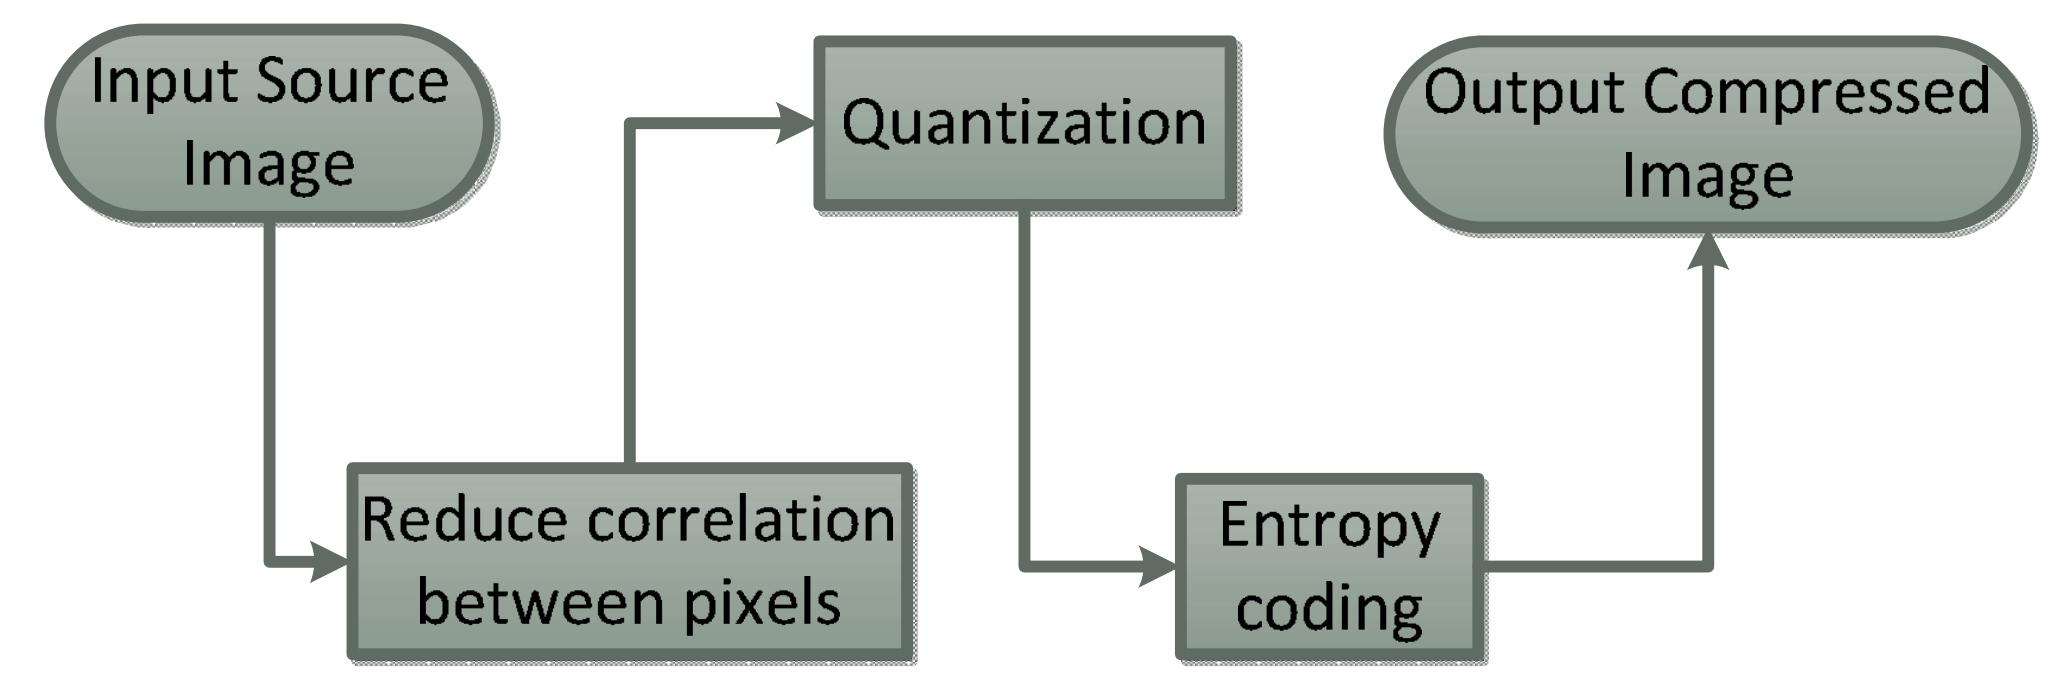
\includegraphics[width=0.9\textwidth]{compression system.png}
  \caption{Typical Compression System Architecture from \cite{raid2014jpeg}}
  \label{fig:compression-arch}
\end{figure}

\subsection{Evaluation Metrics}
In order to meaningfully compare different compression systems, we need to have
metrics to objectively compare their results. In image compression, two important
criteria that these metrics need to capture are the level of compression and the
quality of the reconstruction. The most common metrics for both of these criteria
are listed and defined below:

\begin{enumerate}[label=\textbf{(\alph*)}]
  \item \textbf{Compression.} The most common measure for the degree by which an
  image was compressed is perhaps the most obvious of just utilizing the compression
  ratio CR defined as follows\cite{sayood2017introduction}:
  \[
    CR = \frac{\text{Size}_\text{compressed}}{\text{Size}_\text{original}}
  \]
  \item \textbf{Quality of Reconstruction.} A commonly accepted method of measuring
  the quality of image reconstruction is that of peak signal-to-noise ratio (PSNR).
  To define the PSNR between the original image $I$ and compressed representations $C$
  using the common error metric of the mean square error (MSE) as follows:
  \[
    \text{PSNR}(I, C) = 10 \log_{10}(\frac{\max_{i, j}(I_{ij})^2}{\text{MSE}(I, C)})
  \]

  where MSE is defined as
  \[
    \text{MSE}(I, C) = \frac{1}{m \cdot n} \sum_{i = 1}^m \sum_{j = 1}^n (I_{ij} - C_{ij})^2
  \]
\end{enumerate}

\section{Background}
The following section will provide a brief exposition to the theory behind the methods
utilized in the experiment section.

\subsection{Color Specification}
One of the most commonly utilized tricks to improve the performance of image compression
systems is to store images using YUV color coordinates rather than RGB coordinates.
Rather than storing the red, green, and blue components of the different pixels in 
an image, descriptions of pixels in YUV coordinates are made out of a luminance (Y)
and chrominance (U, V) components. The reason this scheme is useful is because the
luminance plays a much more crucial role than color in the way the human-eye 
perceives light. Separating the luminance and chrominance components therefore allows
us to discriminate how much information we throw away from each of these components
based on how much they affect the way we perceive them. \cite{podpora2014yuv}

We can relate YUV and RGB color coordinates according to the following formula:

\[
  \begin{pmatrix} Y \\ U \\ V \end{pmatrix} = 
  \begin{pmatrix}
    0.299 & 0.587 & 0.114 \\
    -0.169 & -0.334 & 0.500 \\
    0.500 & -0.419 & -0.081
  \end{pmatrix}
  \begin{pmatrix} R \\ G \\ B \end{pmatrix} + 
  \begin{pmatrix} 0 \\ 128 \\ 128 \end{pmatrix}
\]

\subsection{Transform Coding}
At a fundamental level, a transform coding of an $m$ by $n$ matrix $A$ can be thought
as a factorization of the form:
 \[
   A = U_l C U_r^\top
 \]
 where $U_l$ and $U_r$ are unitary matrices and C is an n by n matrix coefficient
 whose form depend on the transform. As such, a transform is reversible and the
 coefficient matrix can be computed as:
 \[
   C = U_l^\top A U_r
 \]
 Two prominent examples of transforms are the discrete cosine transform (DCT) and
 singular value decomposition (SVD) and are briefly described below. \cite{dapena2002hybrid}

\subsection{Singular Value Decomposition}
One of the most famous factorizations that follow the above form is that of the
singular value decomposition. In SVD, a matrix A with rank $r$ is decomposed into 
two eigenvector matrices ($U_l = U$ and $U_r = V$) and a non-negative diagonal
matrix $C = \Sigma$. A possible approach to compute these matrices is to calculate
the eigenvalues $\lambda_i$ of the matrix $A^\top A$ and then solving the system
of equations defined by finding the null space of all matrices in the form
\[
  A^\top A - \lambda_i~\text{ s.t. } 0 \leq i \leq r
\]

In practice, however, iterative methods such as the Householder Method or the QR 
iteration are used.\cite{trefethen1997numerical}

\subsection{Discrete Cosine Transform}
One of the most widely used transform coding methods by far is that of the discrete
cosine transform (DCT). Most notably, it has been part of the compression algorithm
of choice for the popular image format JPEG. Some of the properties that make DCT
a great transform choice for image compression include: (1) It has a fixed set of
basis functions, so there is no need to transmit the basis used. (2) It has the 
ability to reduce the compression artifact effect (i.e. visible block boundaries).
(3) It is able to compress energy into low frequencies in image data. \cite{reininger1983distributions}
\cite{ahmed1974discrete}

More formally, we can use the framework of \textbf{2.2} to define DCT as a 
factorization of the form

\[
  A = U_L C U_R^\top
\]

where the orthogonal matrices $U_L$ and $U_R$ are defined as 

\begin{align*}
  U_{Lij} &= \begin{cases}
    \sqrt{\frac{1}{m}} & i = 1 \\
    \sqrt{\frac{2}{m}} \cos(\frac{\pi (2j - 1)(i - 1)}{2m}) & 2 \leq i \leq m
  \end{cases} \\
  U_{Rij} &= \begin{cases}
    \sqrt{\frac{1}{n}} & i = 1 \\
    \sqrt{\frac{2}{n}} \cos(\frac{\pi (2j - 1)(i - 1)}{2n}) & 2 \leq i \leq n
  \end{cases}
\end{align*}

The fact that $U_L$ and $U_R$ are independent of the matrix to be encoded $A$ and
can thus be inferred without explicitly being included in the encoding of $A$
give DCT a huge advantage in terms of the the compression ratio it can achieve
to transforms like SVD where the normal basis that makes up $U_L$ and $U_R$ are
dependent on $A$ and need to be included for proper decoding.

\subsection{Quantization}
After the transform has been applied, we can utilize our knowledge about the mechanism
of the transform as well as our perception to selectively discard information that
we believe to be unimportant to reasonably reconstructing the original input. 

In SVD, this can easily be done by selecting the rank $r' \leq rank(A)$ by which to 
approximate the original matrix. After choosing $r'$ we can throw away any columns
of $U_L = U$ and $U_R = V$ that have an index greater than $r'$ and prune $C = \Sigma$ to
the square matrix $\Sigma[1:r', 1:r']$. With respect to the Frobenius norm, this
resultant matrix is the closest matrix with the restriction $rank \leq r'$ to the 
original matrix A. \cite{trefethen1997numerical}

For DCT, quantization aims to reducing the coefficients of the least important (high)
frequencies to zero. This approximation takes advantage of the fact that the high
frequencies components of images are often inconsequential to the way that we
perceive them. To perform these quantization, we have defined fixed standard matrices 
$Q$ that determine how relevant each frequency coefficient is. The quantized coefficients, $K$,
are then calculated by a scaling followed by rounding as follows: 

\[
  K_{ij} = \text{round}(\frac{C_{in}}{Q_{ij}})
\]

The JPEG standard provides the following two tables for the quantization of luminance
and chrominance respectively: \cite{sangwine2012colour}

\begin{align*}
  Q_Y &= \begin{pmatrix}
    16&11&10&16&24&40&51&61 \\
    12&12&14&19&26&58&60&55 \\
    14&13&16&24&40&57&69&56 \\
    14&17&22&29&51&87&80&62 \\
    18&22&37&56&68&109&103&77 \\
    24&35&55&64&81&104&113&92 \\
    49&64&78&87&103&121&120&101 \\
    72&92&95&98&112&100&103&99
  \end{pmatrix} \\
  Q_C &= \begin{pmatrix}
    17&18&24&47&99&99&99&99 \\
    18&21&26&66&99&99&99&99 \\
    24&26&56&99&99&99&99&99 \\
    47&66&99&99&99&99&99&99 \\
    99&99&99&99&99&99&99&99 \\
    99&99&99&99&99&99&99&99 \\
    99&99&99&99&99&99&99&99 \\
    99&99&99&99&99&99&99&99
  \end{pmatrix}
\end{align*}

Once the data has been quantized, it is necessary to define an ordering to the 
data so as to define how it is to be stored. In the case of transforms like DCT 
where only the coefficients need to be packed, it is customary to encode the coefficients
using a zig-zag pattern like the one shown in figure \ref{fig:zigzag}.

\begin{figure}[tbhp]
  \centering
  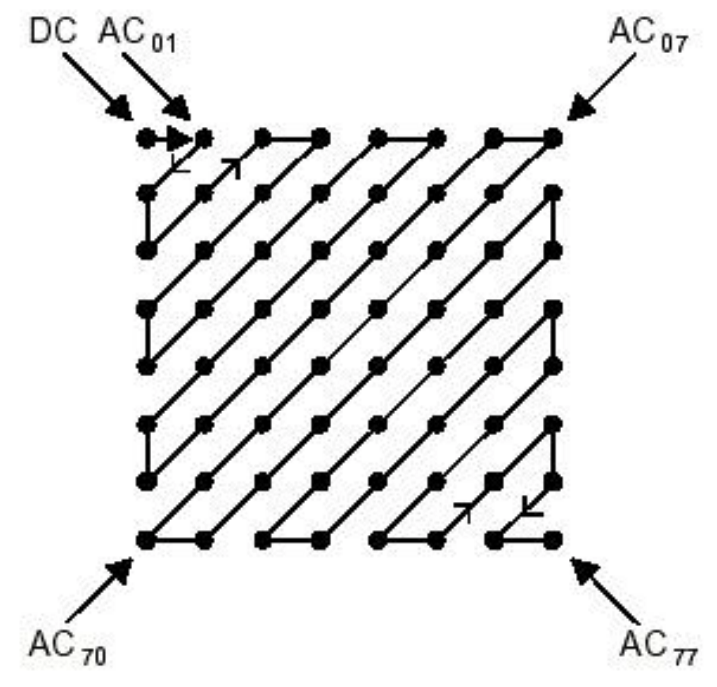
\includegraphics[width=0.5 \textwidth]{zigzag}
  \caption{Diagram of Zig-zag sequencing from \cite{raid2014jpeg}}
  \label{fig:zigzag}
\end{figure}

This ordering takes advantage that low-frequencies normally have non-zero coefficients 
and high-frequencies tend to have zero-coefficients. Packing the zero-coefficients
together allows for better compression using an entropy-coding algorithm such as 
Huffman Coding.

\subsection{Block Algorithms}
A common technique when designing image and video compression systems is that of
using a block-based approach to coding. Rather than applying a transform directly
on the entire image, the image is first divided into smaller blocks or sub-matrices
to which the transform is then applied. This approach facilitates taking advantage of
spacial redundancies often encountered images \cite{ahmed1974discrete}. For DCT, 
it is customary to utilize square blocks of size 8.

\subsection{Huffman Coding}
As depicted in figure \ref{fig:compression-arch}, after the quantization step,
further lossless compression is obtained using a form of entropy coding. One of the
widely used algorithms used for this purpose was suggested by David Huffman in the
paper ``A Method for the Construction of Minimum-Redundancy Codes'' \cite{huffman1952method}.

The algorithm can efficiently create encodings for the symbols utilized in the original
data given a list of frequencies for each symbol. If the frequencies of the symbols
used are ordered, it is possible to design an appropriate encoding in linear time
as follows:

\begin{algorithm}
  \caption{Huffman Encoding}
  \label{alg:huffman}
  \begin{algorithmic}[1]
  \STATE{For each symbol $s_i \in S$, create a leaf vertex $v_i$}
  \STATE{Create two priority queues $Q_1, Q_2$}
  \STATE{Enqueue all $v_i$ in the first queue according to their symbol frequency $f(v_i)$ 
  in increasing order}

  \WHILE{$|Q_1| + |Q_2| > 1$}
  \STATE{Dequeue the lowest two vertices of the queues by examining the fronts of
  both queues}
  \STATE{Create a new inner vertex that has the two dequeued as child nodes and arbitraryly
  label one as the `0'-child and the other as the `1'-child. The frequency of this new node will
  be defined as the sum of the frequencies of its two children.}
  \STATE{Enqueue the new node into the rear of $Q_2$}
  \ENDWHILE
  \RETURN {The single remaining root-vertex.}
  \end{algorithmic}
\end{algorithm}

The encoding for a given symbol is then given by the path taken from the root node
to the leaf vertex that contains the symbol in question. This scheme produces a 
code with an optimal weighted average code length as defined by the frequencies of the symbols. \cite{huffman1952method}.

\section{Experiments}
The experiments carried out consisted of compressing the photo shown in figure \ref{fig:benchmark} using
a block size of 8 with both SVD and DCT. For each trial, the compression ratio
to the original image was recorded and the quality of reconstruction was measured
using PSNR.

\begin{figure}
  \centering
  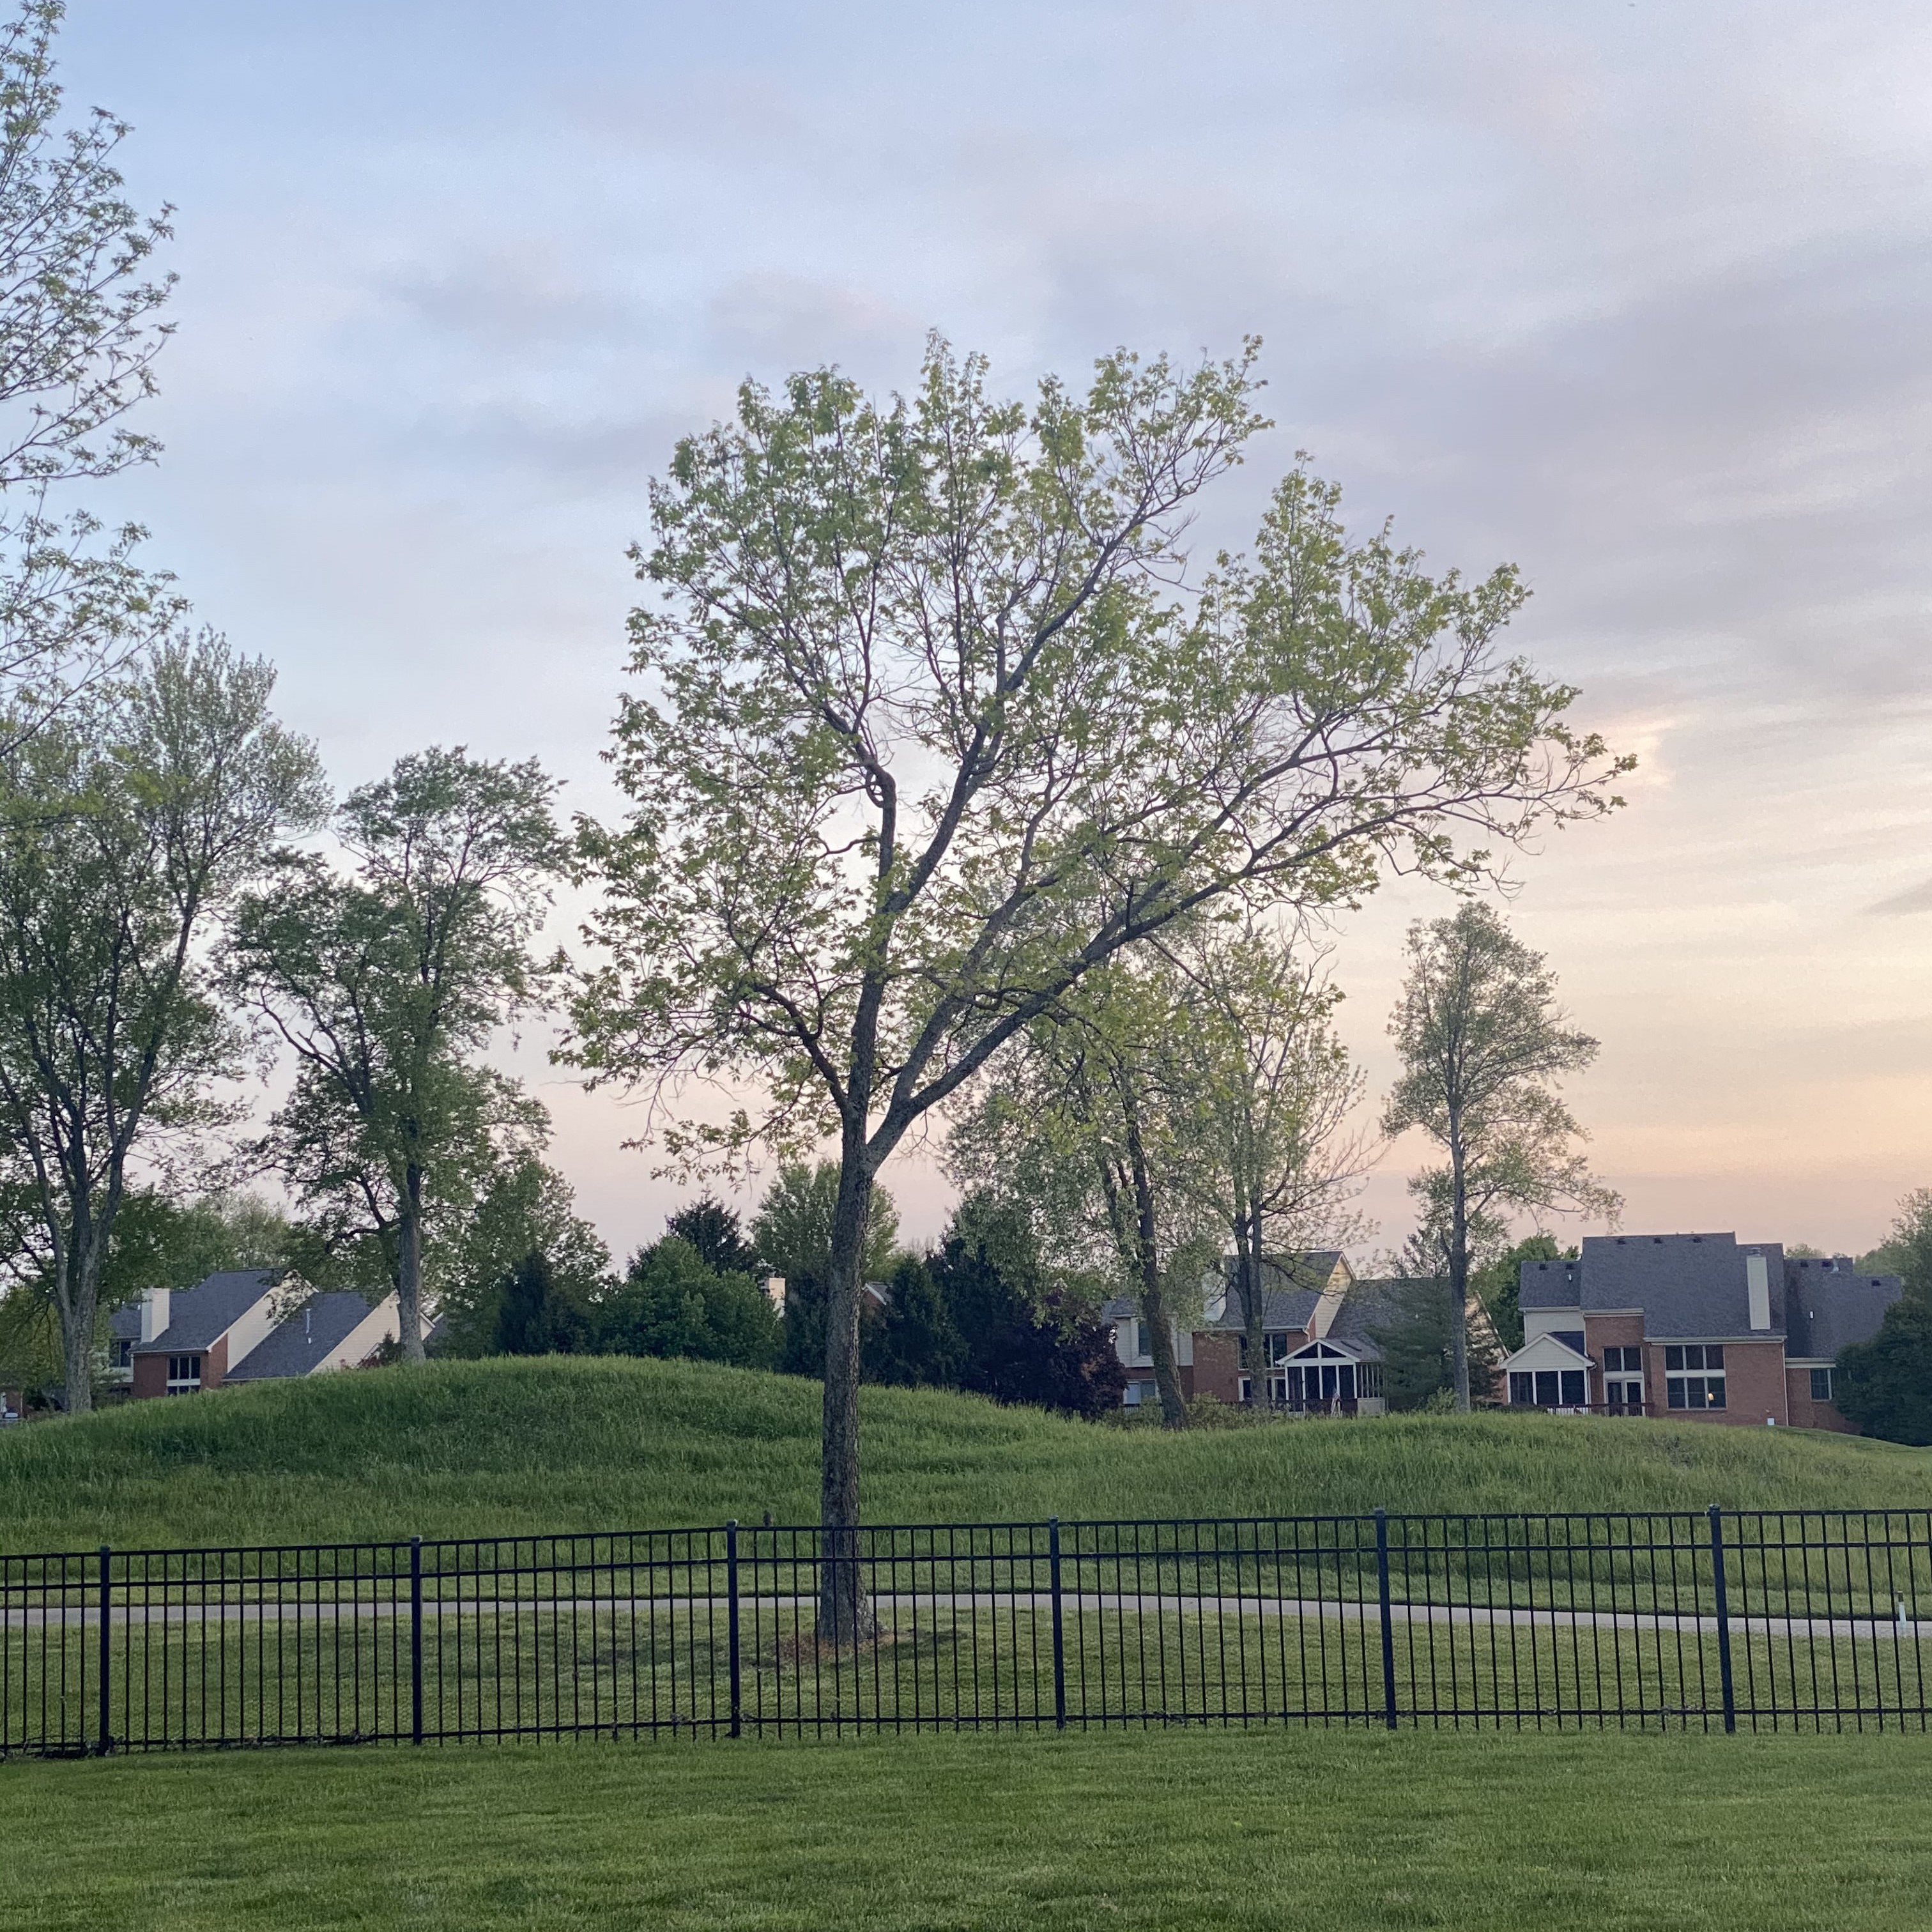
\includegraphics[width=0.5 \textwidth]{backyard.jpg}
  \caption{Benchmark Image}
  \label{fig:benchmark}
\end{figure}

\subsection{Image Quality}
To control the compression ratio obtained with DCT, we varied the multiplication
coefficient by which the quantization table given in \textbf{section 2.5} was 
multiplied prior to quantization. The multiplication coefficient was varied from 
0.01 to 1.0 with a resolution of 0.01.

In the other hand, for SVD, controlling the compression was done via placing a
restriction on the fraction of the total value of the singular components that it used in
its factorization. For example, if the limit was set to $f$, then it must be true that
$$f \leq \frac{\sum_i^{r'} \sigma_i}{\sum_i^r \sigma_i}$$
where $r$ is the original rank and $r'$ is the rank of the factorization used.

For the experiments involving SVD, the utilized fraction was varied from 0.75 to 1.0
with a resolution of 0.01.

\begin{figure}[H]
  \centering
  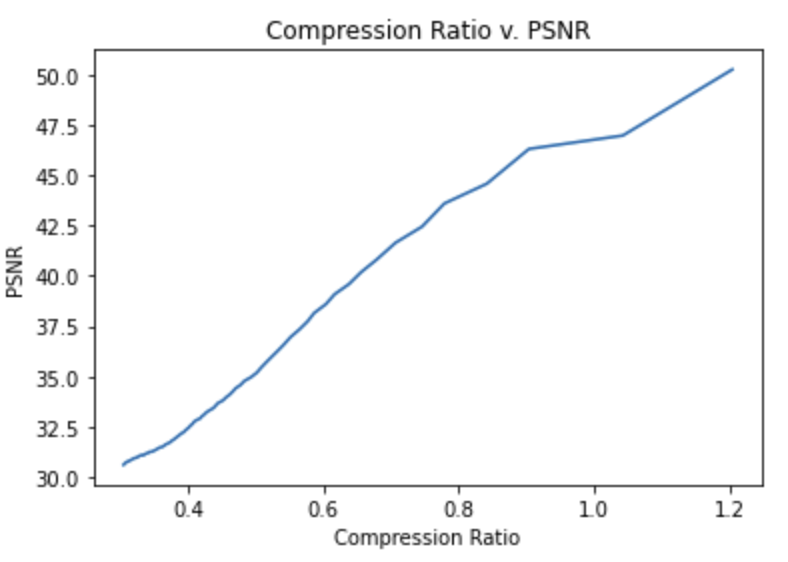
\includegraphics[width=0.5 \textwidth]{dct qual.png}
  \caption{Quality of DCT Reconstruction v. Compression Ratio}
  \label{fig:dctqual}
\end{figure}

\begin{figure}[H]
  \centering
  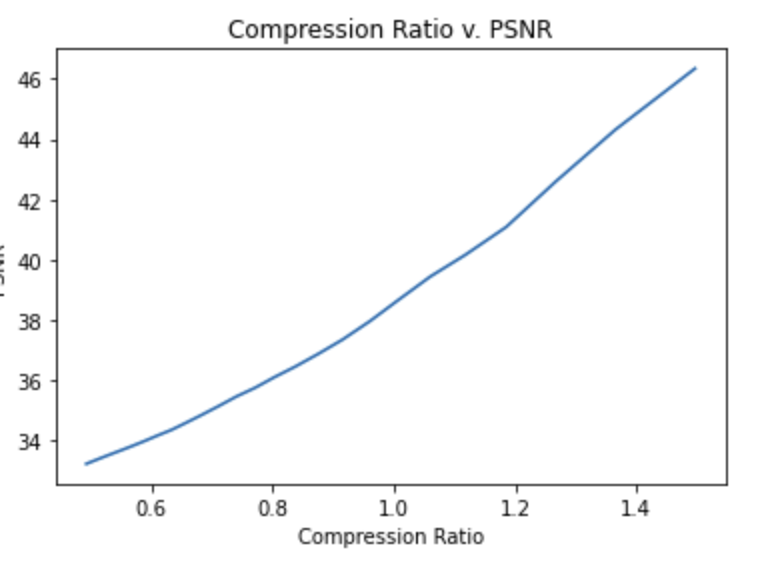
\includegraphics[width=0.5 \textwidth]{svd qual.png}
  \caption{Quality of SVD Reconstruction v. Compression Ratio}
  \label{fig:svdqual}
\end{figure}

As shown by figures \ref{fig:dctqual} and \ref{fig:svdqual}, it seems to be the case
that, for comparable levels of compression, the reconstruction quality of 
DCT is superior to that of using SVD. This is consistent with
the discussion of \textbf{section 2.4} because SVD needs to encode the basis for 
its transform while the DCT does not.

\section{Conclusion}
With the amount of information that we constantly encounter in today's Digital Age
image compression has become a fundamental part of the systems we use. In this paper,
we went over the fundamental components that make up a lossy image compression system
such as the one used in the JPEG standard. Additionally, we numerically compared 
the compression achieved by utilizing similar compression systems; one based on SVD
and the other on DCT and empirically observed that DCT is able to achieve better 
quality reconstructions for a given compression ratio.

\pagebreak
\bibliographystyle{siamplain}
\bibliography{references}
\end{document}
